\chapter{\label{chp:intro} Neutrino Physics}


Since its original inception in the 1930s, neutrino physics has developed into a robust field of high energy physics.  The neutrino was theorized in the 1930s by Wolfgang Pauli, rigorously incorporated into the theory of beta decay by Enrico Fermi \cite{Fermi}, and first detected in 1956 by Clyde Cowan and Frederick Reines \cite{Cowan:1992xc}.

Originally, the neutrino was postulated to preserve conservation of momentum in the theory of beta decay, where a nucleon such as a neutron is converted to a proton by emitting an electron and a neutrino:
\begin{equation}
\label{beta_decay}
n \rightarrow p^+ + e^- + \nuebar
\end{equation}

The reaction above is actually an example of a weak interaction happening at the quark level, where one of the neutron's down quarks converts to an up quark through the emission of a $W^-$.  Unfortunately, the neutrino is a very weakly interacting particle, so the direct observation of both the electron and the neutrino from a $\beta$ decay reaction was, and still is, impossible.  

For the detection of the neutrino, Cowan and Reines used a very similar reaction to beta decay, but instead of producing a neutrino this reaction absorbs a neutrino and emits a neutron and a positron:
\begin{equation}
\label{inverse_beta_decay}
p^+  + \nuebar \rightarrow e^- + n 
\end{equation}

Unlike neutrinos, neutrons and positrons are relatively easy to observe, so Cowan and Reines simply exposed a large sample of protons to a very large blast of neutrinos.  Practically, this meant building a detector near a high intensity source of neutrinos, which they did: they exposed large tanks of water to the neutrino flux of a nuclear reactor at the Savannah River plant, in Georgia.  The neutrinos coming to their detector (actually, {\em anti}-neutrinos) interacted with the protons and produced a neutron and a positron.  The positron was observed after it interacted by annihilating with an electron in the water tank, producing a pair of gamma particles.  The neutron was detected by it's capture on Cadmium, which was doped in the tank.  The neutron capture also produces a gamma, but it is delayed from the positron's gamma pair.  Cowan and Reines ultimately observed about three neutrinos per hour in their detector.  Conclusively, when the reactor was shut off, they no longer observed neutrinos. 

Since the first discovery of the neutrino, neutrinos and their interactions have played a central role in the development of the standard model of particle physics.  Pauli originally proposed only one neutrino, but not long after his prediction (and before the experimental evidence that confirmed it) other types of neutrinos were postulated.   Since then, 2 other types of neutrinos have been discovered, namely the muon and tau neutrinos \cite{PhysRevLett.9.36},\cite{Kodama:2000mp}. 

Conventionally, neutrinos are symbolized as $\nu_e, \nu_\mu,$ and $\nu_\tau$ corresponding to the 3 flavors of charged leptons.  The charged current interactions of these neutrinos, by exchanging a $W^\pm$ boson, produces an outgoing charged lepton of the same flavor as the incoming neutrino: \nue produces electrons, \nuebar produces anti-electrons, \numu produces muons, etc, such as in Equations~\ref{beta_decay} and \ref{inverse_beta_decay}.  However, neutrinos can also interact via neutral currents, where the outgoing lepton is {\em not} charged.  Instead, the neutrino exchanges a neutral $Z^0$ boson with the target material.  The first observed neutral current interaction is shown in Figure~\ref{fig:gargamelle_nc} \cite{Hasert:1973ff}.

\begin{figure}[htbp]
  \centering
  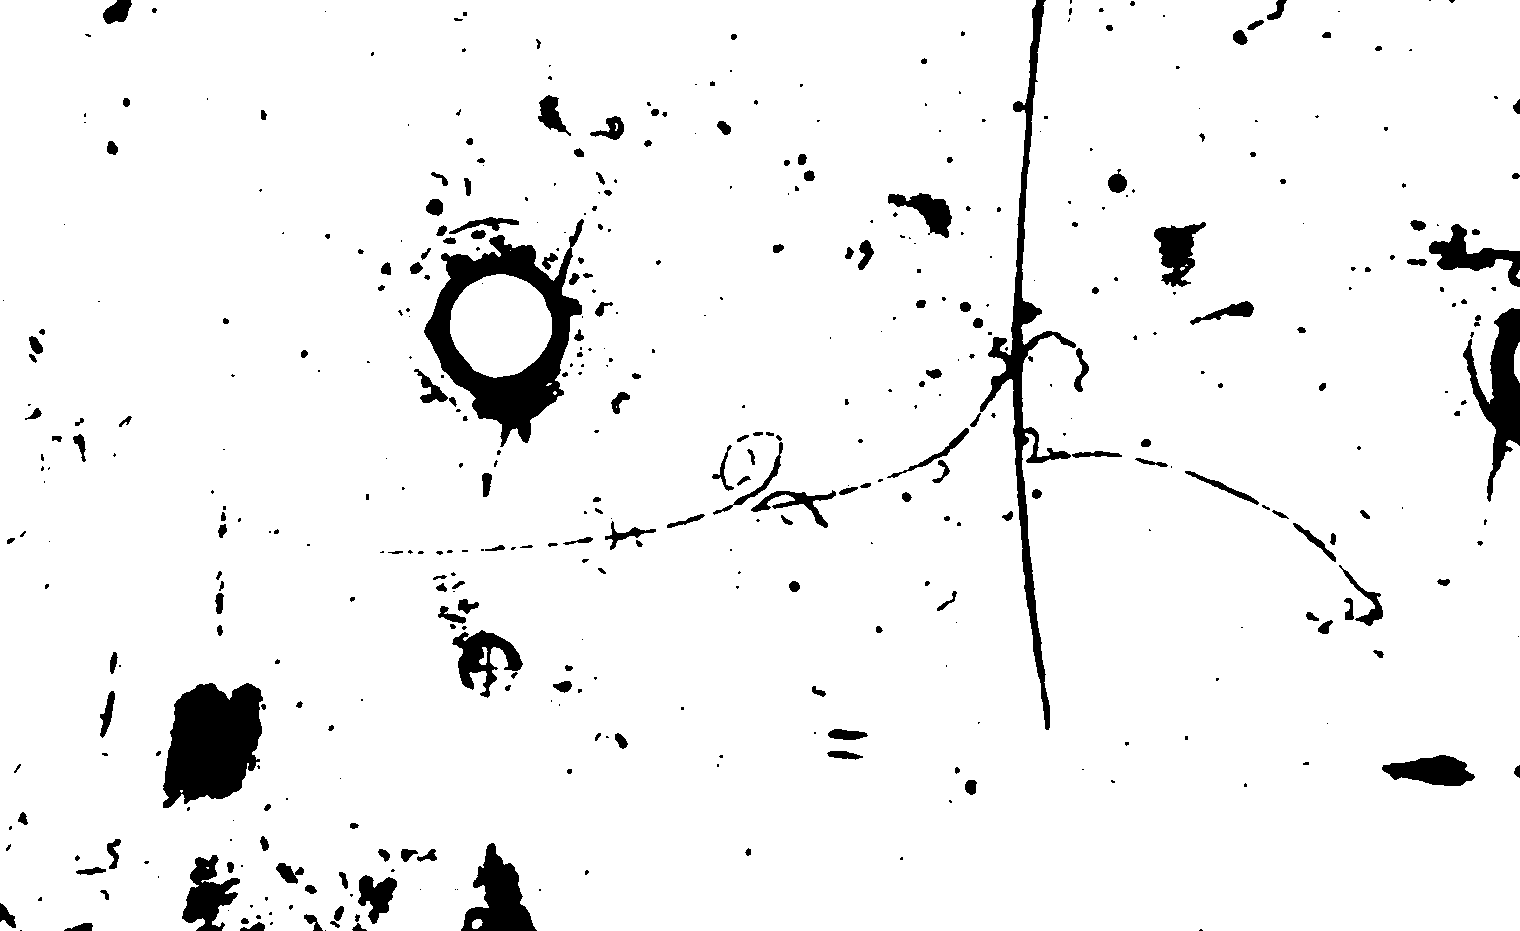
\includegraphics[width=0.95\textwidth]{intro_figures/gargamelle_nc.png}
  \caption[First Observed Neutral Current Neutrino Interaction]{The first observed neutral current neutrino interaction, seen by Gargamelle in 1973.}
  \label{fig:gargamelle_nc}
\end{figure}


Neutrino physics was dramatically altered with the discovery of neutrino oscillations, described below, which opens the door to measurements of CP Violation and possible sterile states of neutrinos.  Since the 1960s until the early 2000s, the field of neutrino physics had an unresolved anomaly known as the Solar Neutrino Problem.  Models of the interactions in the interior of the sun made a definite prediction for the number of electron-flavor neutrinos arriving at Earth \cite{Bahcall:2004pz}, based on well grounded theories of stellar fuel burning.  On the other hand, experiments sensitive to neutrinos observed a significant deficit as compared to predictions \cite{Davis:1968cp}.  It wasn't until the GALLEX/SAGE \cite{Hampel:1997fc, Abdurashitov:1998ne} experiments, along with the Super-Kamiokande experiment \cite{PhysRevLett.81.1562} and the Sudbury Neutrino Observatory \cite{Ahmad:2002jz}, that a solution to the Solar Neutrino Anomaly was found through the mechanism of oscillations: the sun did in fact produce the predicted rate of electron neutrinos, but experiments that were only sensitive to electron neutrinos were unable to detect the muon and tau neutrinos that were produced through the oscillation mechanism.  

The conclusive evidence for neutrino oscillations also implies that neutrinos are not, as was initially believed, massless particles.  However, neutrinos are known to be incredibly light weight, and cosmological constraints imply neutrinos have a summed mass (all three active flavors) of less than 0.23 eV \cite{Abazajian:2011dt, Ade:2013zuv}.  The exact mass of each type of neutrino is unknown still, though experiments are setting lower and lower bounds to directly constrain it \cite{BORNSCHEIN200514, Mertens:2014nha}.

One of the most exciting questions that may be addressed by studying neutrinos is CP violation.  Some theories predict that the current matter/anti-matter imbalance in the observable universe can be explained by CP violation by leptons, such as neutrinos \cite{Nunokawa:2007qh}.  This parameter is directly probable with neutrinos by measuring the difference in neutrino oscillations between neutrinos and anti-neutrinos, as described below.  In particular, the neutrino matter effect \cite{Wolfenstein:1977ue, Mikheev:1986gs} leads to a large observable effect of CP violation in electron neutrinos.

Another intriguing avenue of discovery in neutrino physics is the resolution of short baseline anomalies, which may hint towards the existence of sterile neutrinos.  Experiments have been proposed to probe these anomalies \cite{Antonello:2015lea, Ashenfelter:2015uxt}, and other existing experiments have found ways to investigate short baseline anomalies already \cite{TheIceCube:2016oqi, Adamson:2010wi, MINOS:2016viw, An:2014bik}.

Both for the case of CP violation and the resolution of short baseline anomalies, the detection and measurement of electron neutrinos crucial.  The most promising proposal to measure CP violation, DUNE \cite{Acciarri:2016ooe}, will look for the appearance of electron neutrinos in a primarily muon neutrino beam.  The Fermilab Short Baseline Neutrino Program (SBN Program) \cite{Antonello:2015lea} will similarly be searching for electron neutrinos in a primarily muon neutrino neutrino beam.  The first stage of the SBN Program, \uboone, is already running in Fermilab's Booster Neutrino Beam searching for low energy electron neutrinos.

Both DUNE and the SBN Program rely on high granularity detectors for their neutrino searches, the liquid argon time projection chamber (LArTPC, see Chapter~\ref{chp:lartpcs}).  However, at the time of the publication of this thesis, only one \lartpc in the world has ever observed electron neutrinos.  The ICARUS experiment includes an observation of two electron neutrinos at approximately 20 GeV \cite{Antonello:2013gut}.  On the other hand, the energy of interest to both DUNE and SBN is significantly lower, in the range of 1 GeV.  Therefore, the work presented in this thesis is the first observation of low energy electron neutrinos in a liquid argon time projection chamber.   

\section{Neutrino Sources}

Neutrinos, despite their weak interaction cross section and difficulty to observe, are actually incredibly common on Earth - more than a trillion neutrinos pass through an average sized human hand every second.  By far the most powerful nearby source of neutrinos is from the Sun, produced predominantly in proton-proton fusion.  But, more powerful (and more exotic) sources of neutrinos are known to exist, such as supernova \cite{Dadykin:1987ek, Hirata:1988ad}.  Terrestrially, neutrinos are produced in the geothermal reactions of the Earth's core, and there is large flux of ``atmospheric'' neutrinos produced by the interactions of cosmic particles in the upper atmosphere.  As radioactive elements decay through weak interactions, radioactive material emits neutrinos as well - in fact this can be a quite useful source for calibration of neutrino experiments.

There are also artificial sources of neutrinos, most commonly nuclear reactors.  Though they are less powerful than the Sun, neutrino experiments can get significantly closer to a nuclear reactor than to the Sun, and the local neutrino flux can be quite high.  The most sophisticated artificial source of neutrinos comes from the neutrinos beams produced at accelerator complexes such as Fermilab, CERN, and J-PARC.  Artificial neutrino beams can provide a high intensity source of neutrinos over a large range of energies, and offer many other benefits as well.  

A detailed understanding of the source of neutrinos is vital to the success of every neutrino experiment, and Chapter~\ref{chp:beams} explores neutrino beams in more detail.

% \subsection{Solar Neutrinos}

% \subsection{Atmospheric Neutrinos}

% \subsection{Supernova Neutrinos}

% \subsection{Radioactive Sources}

% \subsection{Reactor Neutrinos}

% \subsection{Neutrino Beams}

\section{Neutrino Oscillations}

Neutrino oscillations \cite{Bilenky:1978nj, Maki:1962mu, Langacker:1988up} are the foundation and the starting point for modern neutrino experiments exploring CP violation and short baseline anomalies, and can be used to probe the mass hierarchy of the neutrinos.  As such, they are fundamentally important to neutrino experiments, so a description of the theory of neutrino oscillations and the experimental evidence is presented here.

\subsection{Neutrino Oscillations - Theory}


Neutrinos, when produced through electro-weak interactions, are produced in flavor eigenstates.  To date, there are known to be three flavors of neutrinos: \nue, \numu, and \nutau.  Each of these neutrinos, as suggested by their name, corresponds to a charged lepton.  The conservation of lepton flavor, in electro-weak interactions, dictates that the number of leptons of a particular flavor is conserved during an interaction.  As an example, the decay of a muon to an electron would violate lepton flavor conservation if not for the presence of neutrinos:

\begin{equation}
\mu^- \rightarrow e^- + \bar{\nu}_e + \nu_\mu
\end{equation}

Lepton flavor violation is not, however, a law of nature.  The most striking evidence for the violation of lepton flavor conservation is neutrino oscillations, though there are hints and proposals that lepton flavor could be violated by charged leptons as well \cite{Bartoszek:2014mya}.  For neutrino oscillations, the violation of lepton flavor is a direct result of the fact that neutrinos in the lepton eigenstates are a superposition of the mass eigenstates of neutrinos:

\begin{equation}
\nu_e = \alpha \nu_1 + \beta \nu_2 + \gamma \nu_3
\end{equation}

where the numerical neutrino states represent the neutrinos with a well defined mass.  It should be noted, from a historical perspective, that in fact neutrinos were originally considered to be zero-mass in the Standard Model.  The discovery of neutrino oscillations instead provided definitive evidence that neutrinos {\bf do} have mass.  From a modern perspective, however, the evidence for neutrino masses is overwhelming.  The interesting phenomenon, then, arise from the fact that neutrinos produce in lepton flavor states do not stay stably in those states.  

The most common way to mathematically describe neutrino oscillations is through the Pontecorvo-Maki-Nakagawa-Sakata matrix \cite{Maki:1962mu, Bilenky:1978nj}, or PMNS matrix:

\begin{equation}
  \left(
  \begin{array}{c}
    \nu_e \\
    \nu_\mu \\
    \nu_\tau \\
  \end{array}
  \right)
  =
  \left(
  \begin{array}{ccc}
    U_{e1} & U_{e2} & U_{e3}  \\
    U_{\mu1} & U_{\mu2} & U_{\mu3}  \\
    U_{\tau1} & U_{\tau2} & U_{\tau3}  \\
  \end{array} 
  \right)
  \left(
  \begin{array}{c}
    \nu_1 \\
    \nu_2 \\
    \nu_3 \\
  \end{array}
  \right)
\end{equation}

In this matrix, under the standard assumptions of neutrino oscillations, the rows and columns are normalize such that the matrix is  unitary: $\sum_{i=1}^3 | U_{\alpha i} | ^2 = 1$, and similarly for the columns.  It's very common for the PMNS matrix to be parameterize in terms of mixing angles: 

\begin{align}
  \left(
  \begin{array}{ccc}
    U_{e1} & U_{e2} & U_{e3}  \\
    U_{\mu1} & U_{\mu2} & U_{\mu3}  \\
    U_{\tau1} & U_{\tau2} & U_{\tau3}  \\
  \end{array} 
  \right)
  = 
  \left(
  \begin{array}{ccc}
    1 & 0 & 0  \\
    0 & \text{cos}\theta_{23} & \text{sin}\theta_{23}  \\
    0 & -\text{sin}\theta_{23} & \text{cos}\theta_{23}  \\
  \end{array} 
  \right)
  &\times \\
  \left(
  \begin{array}{ccc}
     \text{cos}\theta_{13} & 0 & \text{sin}\theta_{13} e^{ - i \delta_{CP}}  \\
     0 & 1 & 0  \\
     -\text{sin}\theta_{13} e^{i \delta_{CP}} & 0 & \text{cos}\theta_{13}  \\
  \end{array} 
  \right)
  &\times \\
  \left(
  \begin{array}{ccc}
    \text{cos}\theta_{12} & \text{sin}\theta_{23} & 0  \\
    - \text{sin}\theta_{23} & \text{cos}\theta_{12} & 0 \\
    0 & 0 & 1  \\
  \end{array} 
  \right)
\end{align}

The value of this expansion is that the individual mixing angles are observable with different experimental setups.  The additional phase, $\delta_{CP}$, is needed if neutrinos violate Charge-Parity symmetry.  Some theories suggest that neutrino violation of CP symmetry is responsible for the matter/anti-matter asymmetry in the Universe (see Section~\ref{sec:future_experiments}).

In general, an experiment probing neutrino oscillations will start with an ensemble of neutrinos prepared in a particular flavor state $\nu_\alpha$:
\begin{equation*}
\nu_\alpha = U_{\alpha 1} \nu_1 + U_{\alpha 2} \nu_2 + U_{\alpha 3} \nu_3
\end{equation*}

The state of the neutrino $\nu_\alpha$ evolves according to the standard time evolution operator, and so at a later time the neutrino state is  
\begin{equation*}
\nu_\alpha (t) = U_{\alpha 1} \nu_1(t) + U_{\alpha 2} \nu_2(t) + U_{\alpha 3} \nu_3(t)
\end{equation*}

where $\nu_{j}(t) = e^{-i ( E_j t - \vec{p} \dot \vec{x})} \nu_j (t)$, using the plane wave solution for the neutrinos.  Since each neutrino has a different mass, the three components of a neutrino flavor state become out of phase as time passes.  Since the neutrino masses are known to be very small, and the neutrinos detected in experiments are typically energies of MeV or higher, all observed neutrinos are ultra-relativistic.  So, the energy expression in the time evolution of the neutrino flavor state can be simplified with $E_j \approx E + \frac{m_j^2}{2E}$.  Therefore, the probability that a neutrino that started in state $\alpha$ will be observed in state $\beta$ at a later time $t$ is:

\begin{equation*}
P_{\alpha\rightarrow\beta} = \left|\braket{\nu_\alpha(t) | \nu_\beta}\right|^2 = \left|\sum_i U_{i\alpha} U_{i\beta} e^{-i t \frac{m_j^2 }{ 2 E}}\right|^2
\end{equation*}

Of course, since neutrinos are ultra-relativistic it is not possible to observe them at a later time in the same location.  Instead, neutrino oscillations searches observe the neutrinos at a distance away from the source.  Assuming the neutrinos travel at the speed of light, so that $L = c t$ (and typically setting c = 1), the useful oscillation probability expression for neutrino experiments is 

\begin{equation*}
P_{\alpha\rightarrow\beta} = \left|\sum_i U_{i\alpha} U_{i\beta} e^{-i m_j^2 \frac{L}{2E}}\right|^2
\end{equation*}

For the case of oscillation between two types of neutrinos, the oscillation probability is often expressed as

\begin{equation}
P_{\alpha\rightarrow\beta} = \text{sin}^2(2\theta)\text{sin}^2\left( \frac{\Delta m^2 L}{4 E} \right)
\end{equation}

As seen in the next section, the sinusoidal characteristic of oscillations is apparent when the neutrinos are presented as a function of $L/E$.

\subsection{Neutrino Oscillations - Experimental Evidence}

Neutrino oscillations have a compelling record of experimental evidence in their favor.  This section provides a brief overview of some of the notable oscillation experiments to date.  A much more complete summary of neutrino oscillations, both theory and experimental evidence, is available from the Particle Data Group \cite{Agashe:2014kda}.

\subsubsection{Solar Neutrino Problem}

The first experimental hint of neutrino oscillations came, retrospectively, with the ``Solar Neutrino Problem.''  The standard Solar model makes a definite prediction for the number of neutrinos produced by the sun \cite{Bahcall:2004pz}, while the observation of Ray Davis and John Bahcall at the Homestake experiment observed only approximately one third of the neutrinos they expected from the Sun.  This observation was subsequently reproduced and confirmed by a number of experiments \cite{Hampel:1998xg, Fukuda:1996sz, Gavrin:2005ks, Anselmann:1992um, Altmann:2005ix, Fukuda:2002pe, Ahmad:2001an, Ahmad:2002jz}.

The many neutrino detectors observing the solar neutrinos produced different measurements of their observed flux, compared to predictions from standard solar models - see Figure~\ref{fig:solar_neutrino_deficit}.  Each experiment, however, observes a different deficit of neutrinos.  However, the experiments searching for solar neutrinos had different minimum thresholds for detection, and the solar neutrino flux is not constant with energy (Figure~\ref{fig:solar_neutrino_flux}).  This strongly implied that the resolution of the Solar Neutrino Problem needed to account for a dependence on neutrino energy, consistent with neutrino oscillations.  Further, the evidence was very strong that the neutrino oscillations in the Sun were affected by the interactions of neutrinos with matter, know as the Mikheev-Smirnov-Wolfenstien (MSW) effect \cite{Wolfenstein:1977ue,Mikheev:1986gs}.

\begin{figure}[htbp]
  \centering
  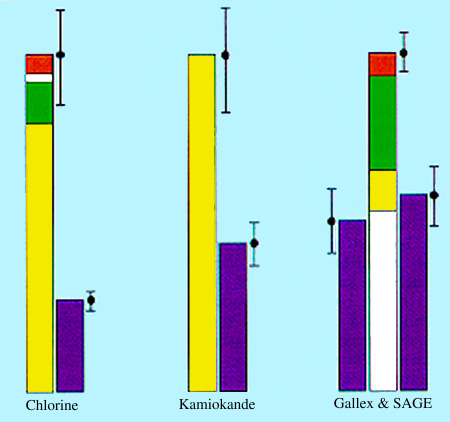
\includegraphics[width=0.45\textwidth]{intro_figures/solar_neutrino_deficit.png}
  \caption[Solar Neutrino Deficit]{Solar neutrino deficit for the different detectors/materials.  Figure from \cite{solar_neutrino_image}.}
  \label{fig:solar_neutrino_deficit}
\end{figure}

\begin{figure}[htbp]
  \centering
  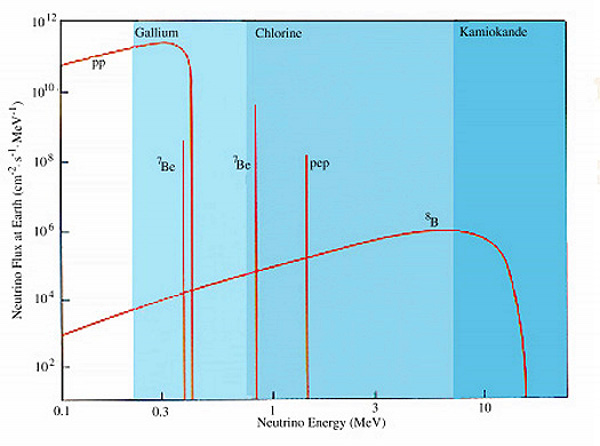
\includegraphics[width=0.65\textwidth]{intro_figures/solar_neutrino_flux.png}
  \caption[Solar Neutrino Flux]{Solar neutrino flux, and the relevant region for the different detectors/materials.  Figure from \cite{solar_neutrino_image}.}
  \label{fig:solar_neutrino_flux}
\end{figure}

Eventually, with the results of experiments such as Super Kamiokande and and SNO, the squared mass separation required to explain the solar neutrino deficit in terms of oscillations was measured as $m_{solar} = 7.5 \times 10^{-5} eV^2$.  This measurement was later confirmed by the KamLAND experiment \cite{Eguchi:2002dm, Araki:2004mb}, who also were able to demonstrate experimentally the sinusoidal dependence of neutrino oscillations, in Figure~\ref{fig:kamland}.  Combined with solar neutrino data, the KamLAND results \cite{Abe:2008aa,Gando:2010aa} indicated that the solar neutrino mass splitting, now understood to be $\Delta m^2_{12}$, is $\Delta m^2{12} = 7.5^{+0.19}_{-0.20} \times 10^{-5} eV^2$, and the oscillation mixing angle is given as $\text{tan}^2(\theta_{12}) = 0.452^{+0.035}_{-0.033}$.

\begin{figure}[htbp]
  \centering
  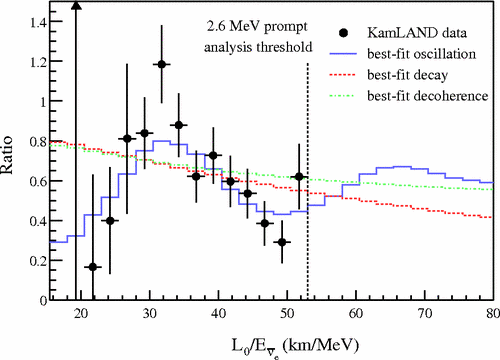
\includegraphics[width=0.45\textwidth]{intro_figures/kamland.png}
  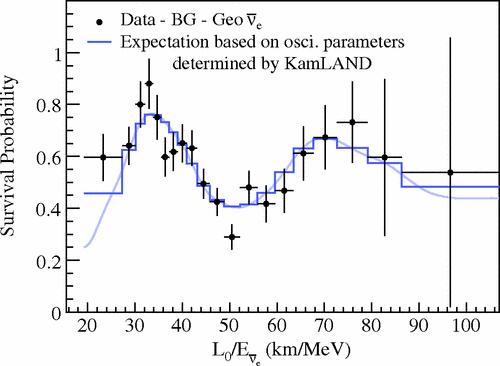
\includegraphics[width=0.45\textwidth]{intro_figures/kamland_highstats.png}
  \caption[KamLAND Oscillation Results]{(Left) Initial oscillation spectrum from KamLAND. (Right) Higher statistics results from KamLAND.  The data are plotted with L=180km, and the data agree well with the best fit oscillation hypothesis. Figures from \cite{Araki:2004mb,Abe:2008aa}.}
  \label{fig:kamland}.
\end{figure}

The resolution of the solar neutrino anomaly set off a cascade of neutrino oscillation searches, including the search for oscillations outside of the solar neutrino regime.  The observation of atmospheric oscillations, in fact, was historically the first direct evidence of neutrino oscillations.

\subsubsection{Atmospheric Neutrinos}

Earth is continuously bombarded with particles in the upper atmosphere, producing (among other things) a flux of neutrinos primarily from the decay of pions and kaons \cite{Honda:2004yz, PhysRevD.70.023006, Plyaskin:2001ku}.  The atmospheric flux is often predicted as a function of zenith angle, and this allows neutrino oscillation experiments to study neutrinos over a very large range of distances: the shortest distances of travel from production are 10s of kilometers, directly above a detector, to $1.2 \times 10^4$ kilometers, from the opposite side of the Earth.  The atmospheric neutrino flux is composed of primarily of \numu, \numubar, \nue, and \nuebar neutrinos in approximately a 2:1 ratio for (\numu + \numubar) : (\nue + \nuebar) \cite{Agashe:2014kda}.

Compelling evidence for the oscillation of atmospheric muon neutrinos was presented by the Super-Kamiokande collaboration in 1998 \cite{PhysRevLett.81.1562}, shown in Figure~\ref{fig:super_k_oscillations}.  Because the Super-Kamiokande detector is unable to distinguish muons from anti-muons, there is no ability to sign select and the oscillation result is presented as a combined oscillation of muon neutrinos and anti-neutrinos.  Because of the distances involved and the energy range of the neutrinos, the solar neutrino mixing is not plausible as an explanation for the oscillation of atmospheric neutrinos.  In addition, the electron neutrino component of the flux is in general agreement with the observed data, assuming no oscillations.  Therefore, the explanation is that atmospheric muon neutrinos oscillate into tau neutrinos.  A subsequent study confirmed the statistical observation of tau neutrinos from atmospheric oscillations, though the tau neutrinos can not be identified on an event-by-event basis \cite{PhysRevLett.110.181802}.  The atmospheric neutrino oscillation suggests a mass splitting that is in the range of $10^{-3} eV^2$, significantly higher than the observed solar neutrino mass splitting.

\begin{figure}[htbp]
  \centering
  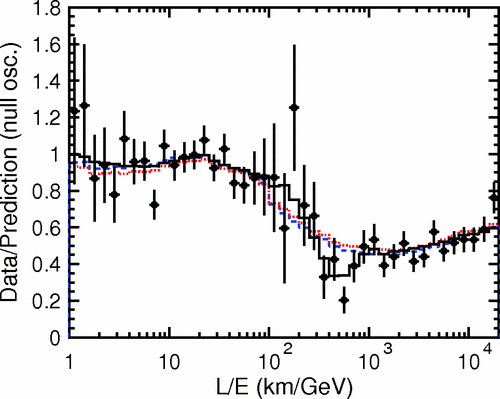
\includegraphics[width=0.65\textwidth]{intro_figures/superk_atmospheric_oscillation.png}
  \caption[Super-K Neutrino Oscillations]{Super-Kamiokande atmospheric neutrino oscillations, as a function of L/E.  L is calculated from the zenith angle of the detected neutrino. Figure from \cite{PhysRevLett.93.101801}.}
  \label{fig:super_k_oscillations}
\end{figure}

\subsubsection{On-axis Neutrino Beams: K2K and MINOS}

The precision measurement of the atmospheric neutrino mixing and mass splitting was determined using long baseline neutrino oscillation experiments with neutrino beams.  The first such experiment, K2K (KEK to Kamiokande), observed oscillations through the disappearance of accelerator produced muon neutrinos \cite{PhysRevD.74.072003}.  MINOS was the second long baseline neutrino oscillation experiment, with a beam of neutrinos from Fermilab traveling to Soudan in Minnesota.  MINOS reported oscillation \cite{PhysRevLett.106.181801} of muon neutrinos as well as muon anti-neutrinos due to the ability of the NuMI beam to run in an anti-neutrino enhanced configuration.  MINOS is a magnetized detector, allowing sign selection of the muons it observes.

The advantage of MINOS and K2K over the results of Super-Kamiokande is that the source of neutrinos is controlled, the energy spectrum is relatively narrow banded (<$E_\nu> = 1.3 GeV$ for K2K), and the length for oscillations is fixed (250 km for K2K, 735 km for MINOS).  Because the parameters of the experiments are more tightly controlled, MINOS and K2K are both able to measure the parameters of atmospheric oscillation with precision.  MINOS's full data set \cite{PhysRevD.86.052007} measures the atmospheric oscillation parameters as $\Delta m^2_A = 2.41^{+0.09}_{-0.10} eV^2$, with $\text{sin}^2(2\theta_A) = 0.950^{+0.035}_{-0.036}$.  In addition, MINOS is able to measure neutrino and anti-neutrino oscillations independently, though the parameters are found to agree for neutrinos and anti-neutrinos within experimental uncertainties.

\begin{figure}[htbp]
  \centering
  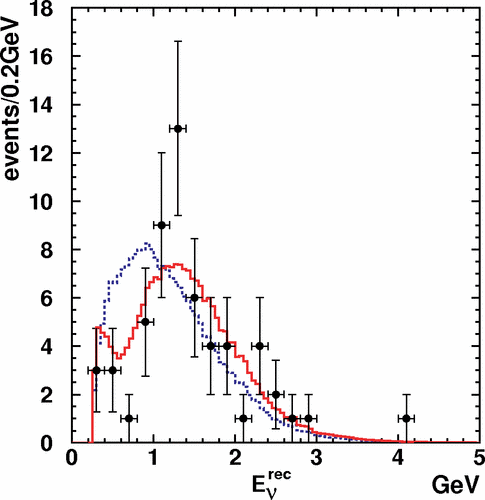
\includegraphics[width=0.45\textwidth]{intro_figures/k2k_oscillations.png}
  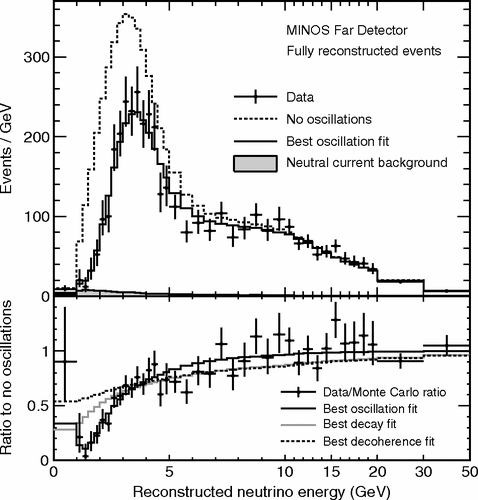
\includegraphics[width=0.45\textwidth]{intro_figures/minos_oscillations.png}
  \caption[MINOS and K2K \numu Oscillations]{(Left) K2K Event spectrum. (Right) MINOS event spectrum.  Both data sets clearly favor the oscillation hypothesis.}
  \label{fig:beam_oscillations}
\end{figure}

\subsubsection{Off-axis Neutrino Beams: T2K, \nova}
As one moves off of the axis of a neutrino beam, the flux from the beam decreases and narrows in energy.  For an oscillation experiment, a mono-energetic and point-like neutrino source is ideal, and an off-axis neutrino beam is closer to this ideal situation.  Both the T2K \cite{PhysRevLett.112.181801} and \nova \cite{PhysRevD.93.051104} experiments utilize this to study neutrino oscillations.  In particular, since \nova is fine grained detector, they are able to observe the appearance of electron neutrinos arising from \numu $\rightarrow$ \nue oscillations \cite{Adamson:2016tbq}.

\begin{figure}[htbp]
  \centering
  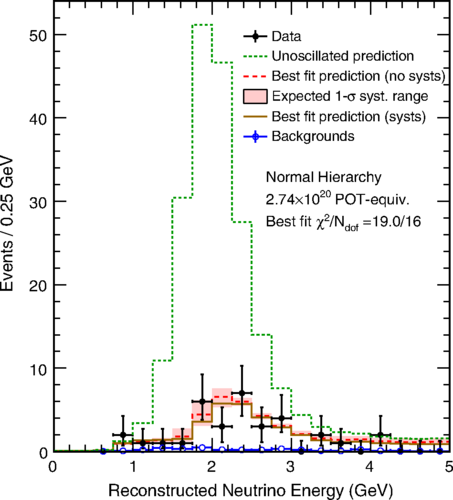
\includegraphics[height=2.5in]{intro_figures/nova_numu.png}
  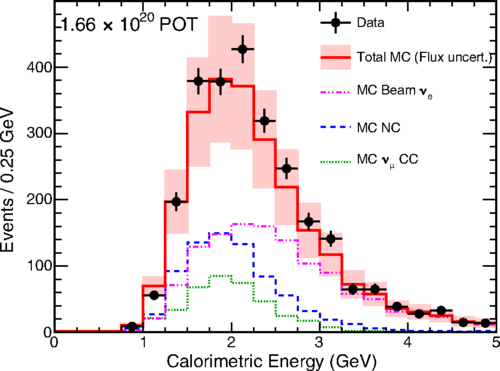
\includegraphics[height=2.5in]{intro_figures/nova_nue.png}
  \caption[\nova Oscillation Results]{(Left) \numu Oscillation results. (Right) \nue appearance oscillation results.  Figures from \cite{PhysRevD.93.051104} and \cite{Adamson:2016tbq}.}
  \label{fig:nova_oscillations}
\end{figure}

\subsubsection{Reactor Neutrinos and $\theta_{13}$}

The three neutrino oscillation paradigm requires three mass splittings (between the three neutrinos) and three mixing angles, however since it's observed that $\Delta m_{solar} = 7.6 \times 10^{-5}$, two of the mass splittings are effectively degenerate.  Measuring the mixing angles is slightly more complicated, however, in the regime where solar neutrino oscillations are not yet relevant the parameter $\theta_{13}$ can be measured effectively.  $\theta_{13}$ can be measured as non-zero from beam experiments such as MINOS, T2K and \nova \cite{PhysRevLett.107.181802, PhysRevLett.116.151806, PhysRevD.88.032002}, but it is directly measurable by searching for electron neutrino disappearance.  Nuclear reactors provide a high intensity flux of electron anti-neutrinos in the $\sim$ MeV range, so an experiment at around 1 km can probe \nuebar disappearance due to mass splittings in the range of $10^{-3} eV^2$.

The first experiment to actively search for \nuebar disappearance due to a nonzero $\theta_{13}$ mixing angle was CHOOZ \cite{Ardellier:2004ui} in France.  CHOOZ found no evidence for non-zero $\theta_{13}$, but set an upper limit on the mixing angle and proposed a follow up experiment to improve sensitivity to lower mixing angles \cite{Ardellier:2004ui}.

In 2012, a suite of experiments measured a non-zero $\theta_{13}$.  Double-CHOOZ \cite{PhysRevLett.108.131801}, Daya Bay \cite{PhysRevLett.108.171803}, and Reno \cite{PhysRevLett.108.191802} all report significant observation of \nuebar disappearance from reactor neutrinos, and Daya Bay and Reno results were at the $5\sigma$ level.  The latest results from Daya Bay \cite{An:2015rpe} show that the measurement of $\theta_{13}$ is at precision levels.  Though it is the last mixing angle measured, it is now the most well known.

\begin{figure}[htbp]
  \centering
  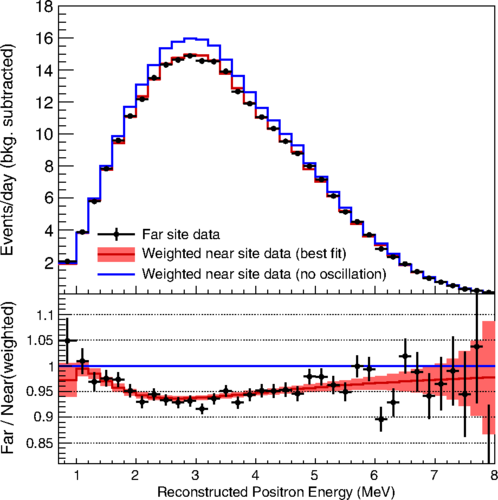
\includegraphics[width=0.45\textwidth]{intro_figures/daya_bay_spectrum.png}
  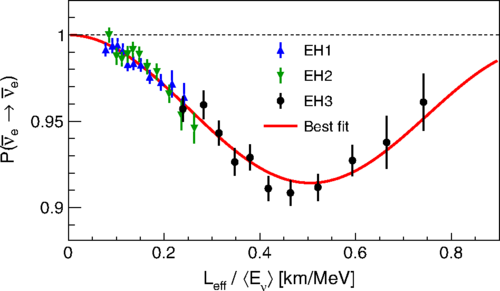
\includegraphics[width=0.45\textwidth]{intro_figures/daya_bay_survival.png}
  \caption[Daya Bay Oscillation Results]{(Left) Daya Bay prompt energy spectrum, showing a clear deficit. (Right) Daya Bay survival probability, showing the characteristic oscillation pattern of neutrino oscillations.}
  \label{fig:daya_bay_oscillations}
\end{figure}

\section{Future Directions in Neutrino Physics}
\label{sec:future_experiments}

Neutrino oscillations are a well established phenomenon.  Despite that, many properties of neutrinos remain elusive.  Some of intriguing puzzles that may be resolved experimentally soon are, for example, the direct measurements of neutrino mass \cite{BORNSCHEIN200514, Mertens:2014nha} by precision measurements of tritium decay.  Other experiments are probing whether or not neutrinos are their own anti-particle by searching for neutrino-less double beta decay \cite{Sisti:2015ayc, Auger:2012ar, 0954-3899-42-11-115201}.  Future experiments will be able to probe the mass heirarchy of neutrinos \cite{Abe:2011ts, Acciarri:2016ooe} as well as search for CP violation in the neutrino sector \cite{Acciarri:2016ooe, Ayres:2004js}.  Undoubtedly, the next decade will produce very exciting results in neutrino physics.

% DUNE and Nova for CP violation, experimental challenges, mass hierarchy, majorana or dirac, 

